%!TEX root = ../main.tex
\section{Query \& ground truth Construction}

\subsection{Synthetic query generation}
In this part, we will discuss how to split large tables and generate the corresponding ground truth.

\noindent \textbf{Choosing Large Tables.} 
To split a base table into multiple small synthetic queries, it is usually necessary to use a large base table with more rows and columns. To achieve this, we sorted all the lake tables by multiplying the number of rows and columns of each table. Tables with rows and columns greater than a certain threshold were selected, and in order to ensure the diversity of synthetic queries, we manually selected tables with differenet semantics as the base tables.

\noindent \textbf{Synthetic Query Construction.} 
To generate syhthetic queries that are relatively realistic, including randomness and a certain level of difficulty. We mainly use two methods to generate synthetic queries for join and union case, which involve horizontal and vertical table splitting.

\noindent \underline{\textit{Union Case.}}  To generate synthetic queries for the unionable case, it is essential for two small tables to share identical columns. Consequently, we generate unionable scenarios by partitioning the original base table both horizontally and vertically, ensuring there is no overlap in rows and varying the extent of column overlap. First, we horizontally split the table into several parts, then randomly select several columns from each part as column overlap. After that, we select the remaining columns that are not duplicate as supplementary columns for each small table, and thus forming the synthetic queries for the union case.

\noindent \underline{\textit{Join Case.}}  Joinable tables must share at least one common joining column, and unlike unionable tables, they should exhibit a substantial row overlap. To construct this case, similar to the method used in the union case we first vertically split the base table into several tables while retaining varying proportions of overlapping columns (e.g., 1 column, 30\% of columns, 50\%, etc.). Furthermore, we horizontally divide the split tables with varying row overlap percentages (in our case,20\%, 35\%, 50\%, etc.). 

\noindent \textbf{Ground Truth Generation.} 
During the process of constructing synthetic queries, ground truth are also generated accordingly.
\noindent \underline{\textit{Union Case.}}  
As mentioned above, we first divide the base table horizontally into different parts, and then select some small tables with common columns in each part. As a consequence, these small tables are unionable in pairs, so we mark them as ground truth.
\noindent \underline{\textit{Join Case.}} 
Similarly, when constructing the syhthetic quries for join case, we initially vertically partition the base table into multiple tables, preserving different percentages of overlapping columns (varying from 1 column to 50\% of columns). These overlapping columns and partition tables correspond to the query table and ground truth of the join case respectively.
%+ How to choose large tables.

%+ How to split.

%+ How to generate the ground truth.
\subsection{Basic search for candidate generation}
In this part, for each synthetic or real query, we design a basic search algorithm to retrieve  candidate joinable/unionable tables from the data lake. 

\noindent \underline{\textit{Union Case.}}  
To retrieve the unionable tables from the data lake, it not only requires considering $(\romannumeral1 ).$  the semantics of the corresponding columns in two tables (i.e. only considering the semantics between individual column pairs), but also $(\romannumeral2 ).$ the semantics between two tables (i.e. the relationships and semantics between different columns in the same table),  Therefore, we used multiple methods that consider these two semantics separately to obtain results on the query table. Specifically, we use \starmie,\santos and SATO. After that, we take the union of these results as the candidate tables and label them by experts.

\noindent \underline{\textit{Join Case.}}  
In the case of joining tables, several considerations are essential:$(\romannumeral1).$ the semantics of corresponding columns in both tables. $(\romannumeral2).$ analyzing the relationship between the two tables, $(\romannumeral3).$ ensuring there is an overlap in cell values between the corresponding columns. Consequently, We used method that considers both $\romannumeral1$ and $\romannumeral2$, namely \deepjoin, and method that considers $\romannumeral3$, namely \josie, to obtain candidate tables respectively.

\noindent  \underline{\textit{Number of Candidate Tables.}}  The number of candidate tables we obtained was determined by experts. We first set an accuracy threshold (i.e. 70\%), and then manually judged that when the number of candidate tables reached a certain number, their corresponding accuracy was lower than the threshold we set. At this point, the number of selected tables is the final number of our candidate tables.
%+ How to guarantee high recall

%+ Details

\subsection{Human labeling}
In this part, we ask the human experts to label the candidates for each query. In order to improve the efficiency of experts data labeling, we built a webpage for labeling the ground truth of both join and union case.

%+ Example shown to the experts.

\noindent \textbf{Labeling Interface.} 
The labeling interface we built is shown in the Figure ~\ref{fig:interface}, we demonstrate the interface for union case and the interface for join case is similar. The interface is mainly divided into three parts in a vertical direction. We will further explain how each part works.

\noindent \underline{\textit{Query Table Specification.}}  
As shown in Figure ~\ref{fig:interface}-\raisebox{.3pt}{\textcircled{\hspace{-0.08cm} \raisebox{-.5pt}{1}}}, this section displays a list of query tables to be labeled.  The figure shows a list of ten query tables and the user can select a specific query table, whose information will be dispalyed in Figure ~\ref{fig:interface}-\raisebox{.3pt}{\textcircled{\hspace{-0.08cm} \raisebox{-.5pt}{2}}}.

\noindent \underline{\textit{Metadata of Query Table.}}  When selecting the corresponding query table,  its corresponding information is to be visualized.(see Figure ~\ref{fig:interface}-\raisebox{.3pt}{\textcircled{\hspace{-0.08cm} \raisebox{-.5pt}{2}}}). For example, after the user chooses the first query table, its main information, including the metadata and the table itself  will be shown. We can see that for the query table \cc{XX}, its column names varying from \cc{XX} to \cc{XX}. Furthermore, for column \cc{XX}, it mainly consists of two distinct cell values, namely \cc{XX} and \cc{XX}. These meta information are displayed above the query table as auxiliary information to help users better determine whether two tables can be joined or unioned.

\noindent \underline{\textit{Candidate Table Specification.}} The functions of this part are similar to that of Query Table Specification (see Figure ~\ref{fig:interface}-\raisebox{.3pt}{\textcircled{\hspace{-0.08cm} \raisebox{-.5pt}{3}}}). In this part, users can select a candidate table and get some relevant visualizations they want. For example, when choosing candidate table \cc{XX}, the interface will show its column name and the corresponding range of cell values for each column.

\noindent \underline{\textit{Metadata of Candidate Table.}}  Similarly, this part provides the explanations in plain text for the metadata of a specific candidate table, which will help the users to better understand the meaning of the entire table.  The users can click the “more” button for more visualization details (see Figure ~\ref{fig:interface}-\raisebox{.3pt}{\textcircled{\hspace{-0.08cm} \raisebox{-.5pt}{4}}}).

\noindent \underline{\textit{Labeling Area.}} The users may select a specific query table and its unionable candidate table and further conduct a labeling operation in the labeling area of the interface (see Figure ~\ref{fig:interface}-\raisebox{.3pt}{\textcircled{\hspace{-0.08cm} \raisebox{-.5pt}{5}}}). Suppose that the user chooses the query table \cc{XX} and candidate table \cc{XX}, by clicking the "union" button, the interface will initiate a process to gather labeled data and store it in the backend database. Upon successful labeling, the system will prompt the user for confirmation.


\begin{figure*}[h]
	\centering
	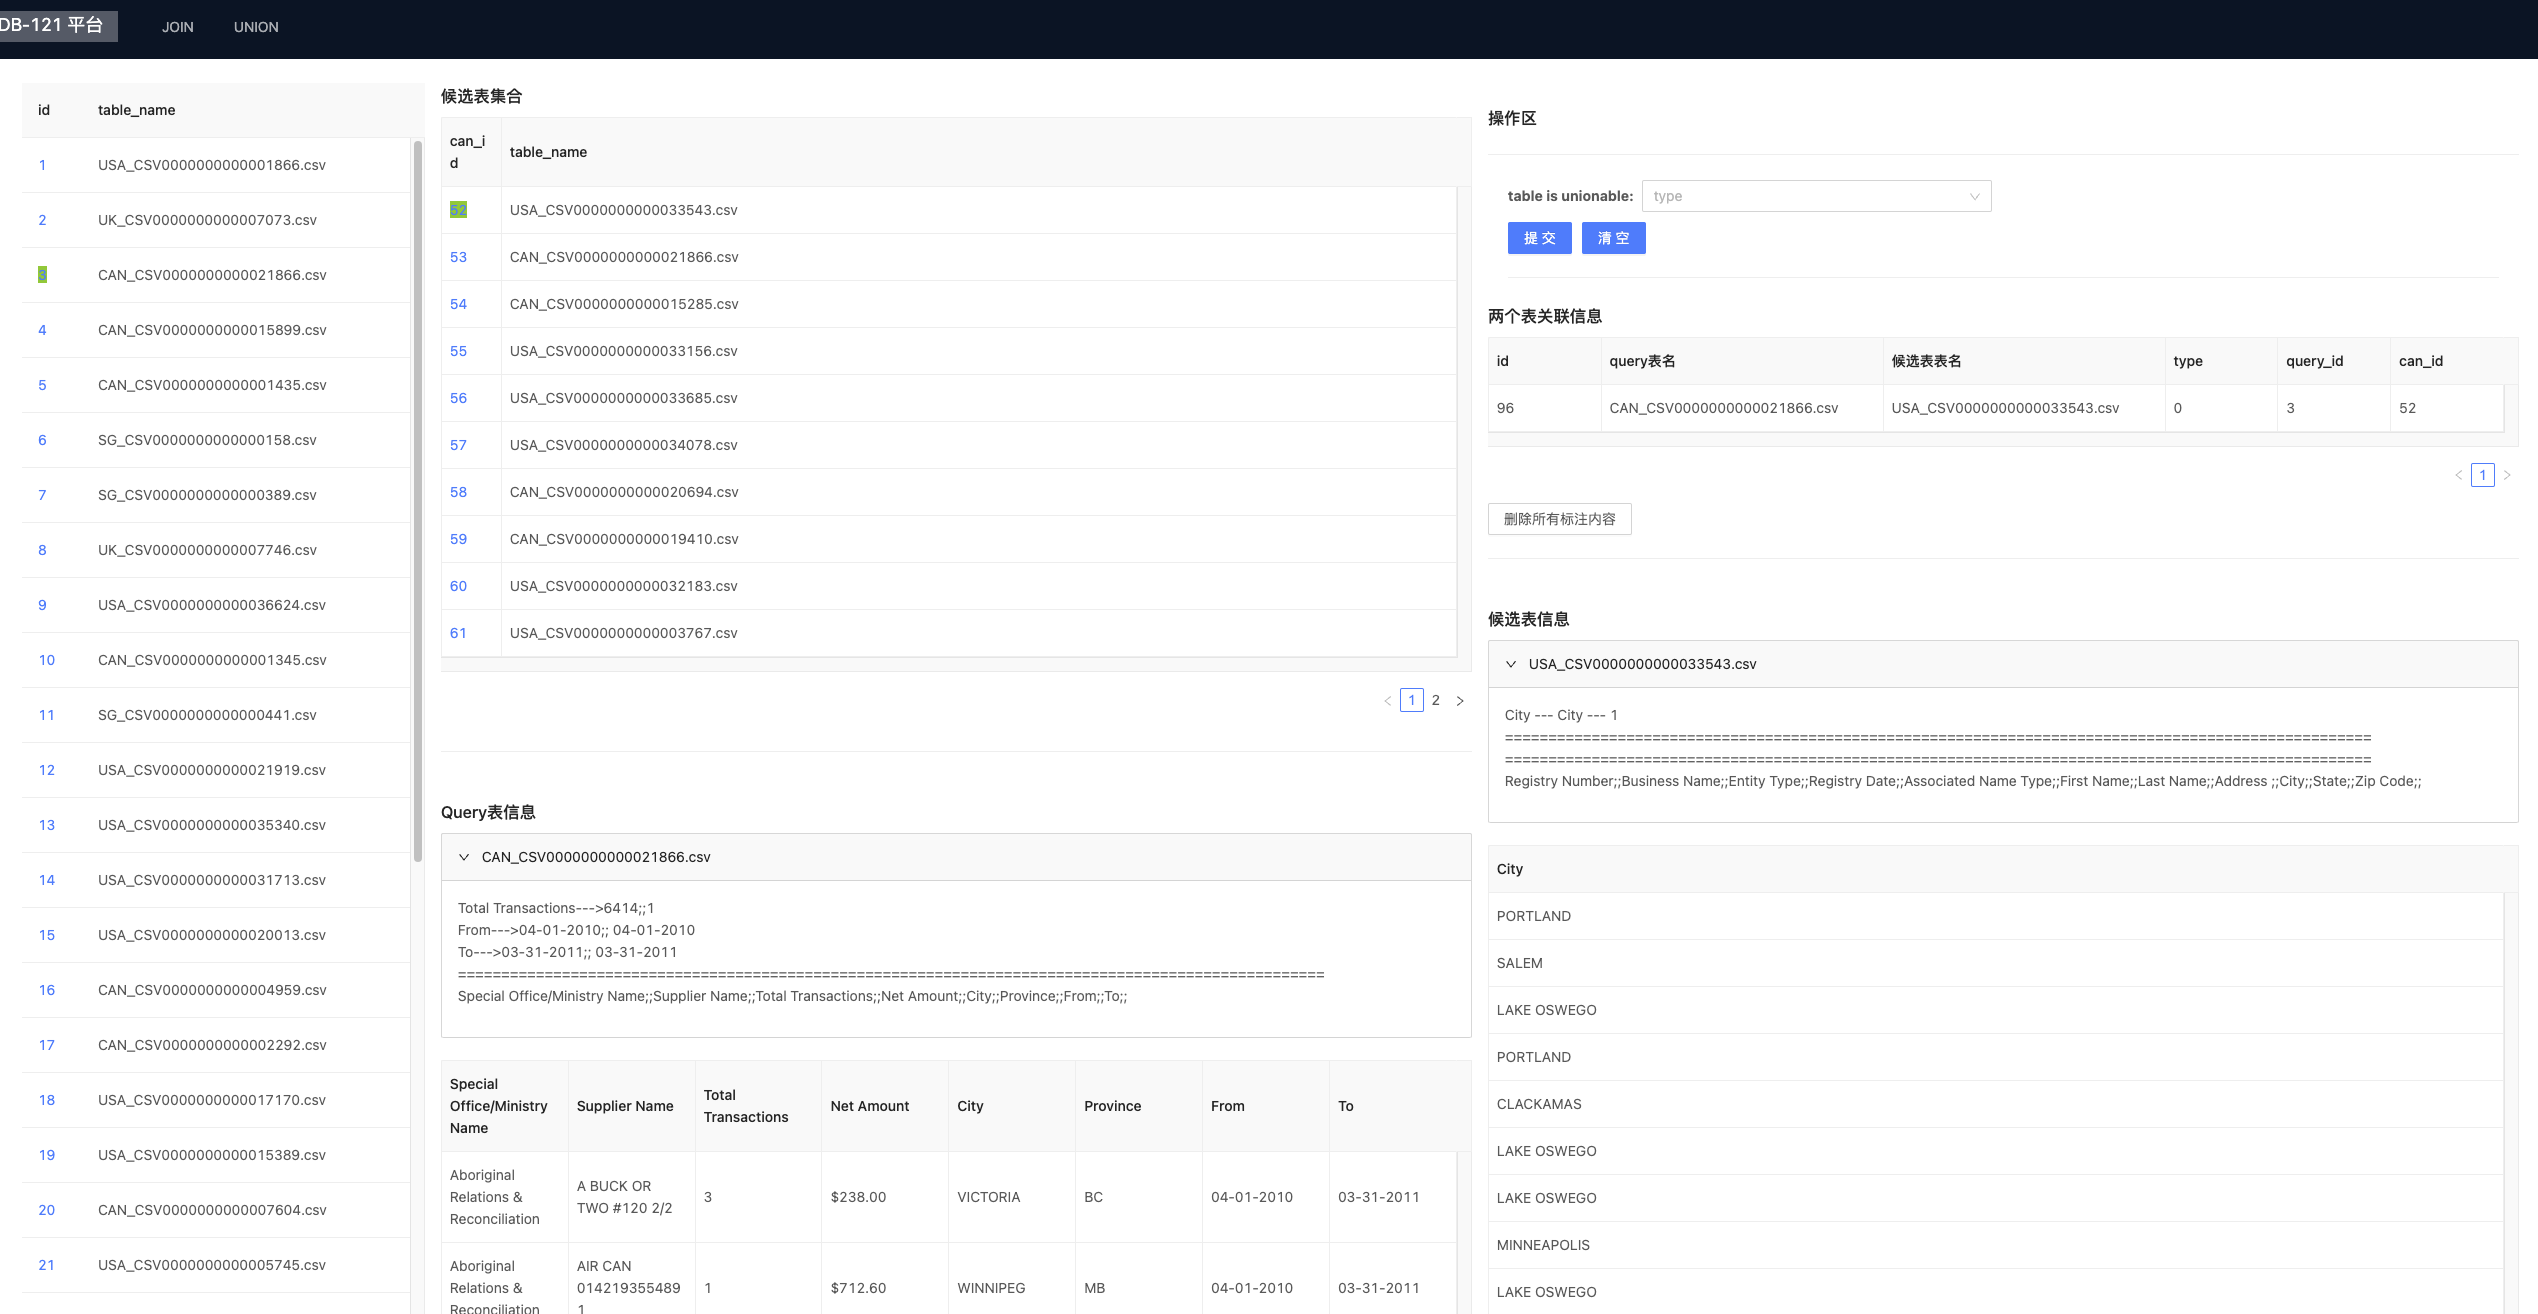
\includegraphics[width=1.0\linewidth]{fig/interface.png}
	\caption{Labeling Interface of Webpage.}
	\label{fig:interface}
\end{figure*}

\noindent \textbf{Labeling Statistics.} 
We have count some statistical information during manual labeling, as show in Table ~\ref{Table:humanLabeling}. For OpenData Large, this dataset has a total of  \cc{XX} query tables to be labeled, with an average of 20 candidate tables matching each query table. Therefore, we have 10 experts and spent a total of approximately \cc{XX} hours completing the labeling work. Similarly, for WebTable Large, we also have 10 experts and spent a total of approximately \cc{XX} hours for labeling. This is because this dataset has \cc{XX} query tables in all that need to be labeled, and each table has an average of 20 corresponding candidate tables.

\begin{table}[t]
	\centering
	\caption{Statistics of Human Labeling.}
	\begin{tabular}{|c|c|c|c|c|c|}
		\hline
		\centering
		Data Lake  & \#-Query Tables & $\#$-People & Time.   \\
		\hline  
		OpenData Small& 914  & 10 & 10h   \\
		\hline
		OpenData Large& 1,448  & 10  &  17.5h   \\
		\hline
		WebTable Small& 1,745   & 10 &  20h  \\
		\hline
		WebTable Large& 2,245  & 10 &  30h  \\
		\hline
	\end{tabular}
	\label{Table:humanLabeling}
	
\end{table}